\documentclass[tikz]{standalone}
\usepackage{pgfplots}
\pgfplotsset{compat=1.15}
\usepackage{mathrsfs}
\usetikzlibrary{arrows,calc}
\usepackage{tkz-euclide}

\pagestyle{empty}

\definecolor{AngleClr}{rgb}{0,0.39215686274509803,0}
\definecolor{ShapeClr}{rgb}{0.6,0.2,0}

\begin{document}

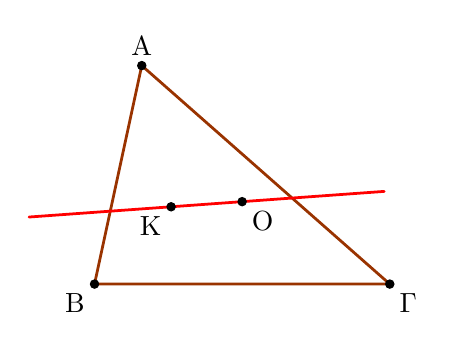
\begin{tikzpicture}[scale=.75]
\tkzSetUpLine[line width=1pt,color=black]
\tkzSetUpPoint[fill=black]

\tkzDefPoints{0/0/B,0.8/3.7/A,5/0/C}

\tkzDefMidPoint(B,C) \tkzGetPoint{MA}
\tkzDefMidPoint(A,C) \tkzGetPoint{MB}
\tkzDefMidPoint(B,A) \tkzGetPoint{MC}

\tkzDefLine[perpendicular=through B](B,C) \tkzGetPoint{BB}
\tkzDefLine[perpendicular=through MC](A,B) \tkzGetPoint{MMC}
\tkzInterLL(B,BB)(MC,MMC) \tkzGetPoint{OB}

\tkzDefLine[perpendicular=through A](A,B) \tkzGetPoint{AA}
\tkzDefLine[perpendicular=through MB](C,A) \tkzGetPoint{MMB}
\tkzInterLL(A,AA)(MB,MMB) \tkzGetPoint{OA}

\tkzInterCC(OA,A)(OB,B) \tkzGetPoints{Br1}{X}



\tkzDefLine[perpendicular=through B](A,B) \tkzGetPoint{BB2}
\tkzDefLine[perpendicular=through MA](B,C) \tkzGetPoint{MMA2}
\tkzInterLL(B,BB2)(MA,MMA2) \tkzGetPoint{OB2}

\tkzDefLine[perpendicular=through A](C,A) \tkzGetPoint{AA2}
\tkzDefLine[perpendicular=through MC](A,B) \tkzGetPoint{MMC2}
\tkzInterLL(A,AA2)(MC,MMC2) \tkzGetPoint{OA2}

\tkzInterCC(OA2,A)(OB2,B) \tkzGetPoints{Br2}{X}


\tkzFillPolygon[fill=white](A,B,C)

\tkzDrawPolygon[color=ShapeClr](A,B,C)

\tkzDefTriangleCenter[circum](A,B,C) \tkzGetPoint{O}

\tkzDefTriangleCenter[circum](O,Br1,Br2) \tkzGetPoint{OO}
\tkzDefTriangleCenter[symmedian](A,B,C) \tkzGetPoint{K}

\tkzDrawSegment[red,add=2.0 and 2.0](O,K)

\tkzDrawPoints[size=3](A,B,C,O,K)

\tkzLabelPoint[above](A){$\mathrm{A}$}
\tkzLabelPoint[below left](B){$\mathrm{B}$}
\tkzLabelPoint[below right](C){$\mathrm{\Gamma}$}

\tkzLabelPoint[below right](O){$\rm O$}
\tkzLabelPoint[below left](K){$\rm K$}

\end{tikzpicture}
\end{document}
